\subsection{测度在开集上的限制. 借助局部数据定义测度}

设 X 是一个局部紧空间，Y 是 X 的一个开集。X 的子空间 Y 是局部紧的，并且每个定义在 Y 上、取值于某个拓扑向量空间 E 且具紧支集的连续函数，都可以通过在 \(\complement \mathrm{Y}\) 上取值 0 而连续地延拓到整个 X；于是可以把空间 \(\mathcal{K}(\mathrm{Y};\mathrm{E})\) 以这种方式等同于 \(\mathcal{K}(\mathrm{X};\mathrm{E})\) 中由紧支集含于 Y 的连续函数所构成的线性子空间。若 \(\mu\) 是 X 上的一个测度，则显然 \(\mu\) 在 \(\mathcal{K}(\mathrm{Y};\mathbf{C})\) 上的限制是 Y 上的一个测度，称为 \(\mu\) 在开子空间 Y 上的限制，或 \(\mu\) 在 Y 上诱导的测度，记作 \(\mu|\mathrm{Y}\) 。依据 §1, No.~5 与 No.~6 ， \(|\mu|\) 、 \(\mathcal{R}\mu\) 与 \(\mathcal{I}\mu\) 在 Y 上的限制分别是 \(|\mu|\mathrm{Y}|\) 、 \(\mathcal{R}(\mu|\mathrm{Y})\) 与 \(\mathcal{I}(\mu|\mathrm{Y})\) 。若 \(\mu\) 是实测度，则依据 §1, No.~5 的公式 (8)， \(\mu^{+}\) 与 \(\mu^{-}\) 在 Y 上的限制分别是 \((\mu|\mathrm{Y})^{+}\) 与 \((\mu|\mathrm{Y})^{-}\) 。

立即可见：若 Y 与 Z 是 X 中满足 \(Y \supset Z\) 的两个开集，且 \(\mu|Y\) 与 \(\mu|Z\) 是 \(\mu\) 在 Y 与 Z 上的限制，则 \(\mu|Z\) 也是 \(\mu|Y\) 在局部紧空间 Y 的开子空间 Z 上的限制。

在 Ch. IV, §5, No.~7 中，我们将把这一定义推广到 Y 是 X 的局部紧子空间的情形。

\pandocbounded{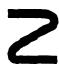
\includegraphics[keepaspectratio]{images/part001_8e0e9629.jpg}}

注意，Y 上的测度未必是 X 上某个测度的限制（参见 Ch. V, §7, No.~2, 命题 3）。

例如，设 Y 是 X = R 中的开区间 {]}0,1{[} ；映射

\[
f \mapsto \int_ {0} ^ {1} \frac {f (x)}{x} d x
\]

是 Y 上的一个测度，因为 \(\mathcal{K}(\mathrm{Y};\mathbf{C})\) 中的每个函数都在 \(\mathbf{R}\) 中 0 的某个邻域上为零。然而这个测度不能延拓为 \(\mathbf{R}\) 上的测度，因为倘若不然，它在函数 \(f\in \mathcal{K}(\mathrm{Y};\mathbf{C})\) （满足 \(\| f\| \leqslant 1\) ）所成之集上的限制将是有界的；而这是不成立的。

不过，我们有下列命题：

命题 1. --- 设 \((\mathrm{Y}_{\alpha})_{\alpha\in\mathrm{A}}\) 是 X 的一个开覆盖，并在每个子空间 \(Y_{\alpha}\) 上给定一个测度 \(\mu_{\alpha}\) ，使得对每个指标对 \((\alpha,\beta)\) ， \(\mu_{\alpha}\) 与 \(\mu_{\beta}\) 在 \(Y_{\alpha}\cap Y_{\beta}\) 上的限制相同。在这些条件下，存在 X 上唯一的测度 \(\mu\) ，使得它在 \(Y_{\alpha}\) 上的限制等于 \(\mu_{\alpha}\) ，对每个指标 \(\alpha\) 均是如此。

首先证明每个函数 \(f \in \mathcal{K}(\mathrm{X};\mathbf{C})\) 都可写成有限和 \(f = \sum_{i} f_{i}\) 的形式，其中对每个函数 \(f_{i} \in \mathcal{K}(\mathrm{X};\mathbf{C})\) ，存在一个指标 \(\alpha_{i}\) 使 \(\operatorname{Supp}(f_{i}) \subset \mathrm{Y}_{\alpha_{i}}\) 。若 \(\mathrm{K} = \operatorname{Supp}(f)\) ，则存在有限个指标 \(\alpha_{i} (1 \leqslant i \leqslant n)\) 使诸 \(\mathrm{Y}_{\alpha_{i}}\) 构成 \(\mathrm{K}\) 的一个覆盖；设 \(h_{i} (1 \leqslant i \leqslant n)\) 是 \(\mathrm{X}\) 到 {[}0,1{]} 中的连续映射，使得 \(h_{i}\) 的支集是紧的且含于 \(\mathrm{Y}_{\alpha_{i}}\) （对 \(1 \leqslant i \leqslant n\) ），并且 \(\sum_{i=1}^{n} h_{i}(x) = 1\) 在 \(\mathrm{K} (\S 1, \text{No. 2, Lemma 1})\) 上成立；函数 \(f_{i} = f h_{i}\) 即合要求。这首先表明：若存在满足要求的测度 \(\mu\) ，则它是唯一的，因为对每个有限和 \(f = \sum_{i=1}^{n} f_{i}\) （其中 \(f_{i} \in \mathcal{K}(\mathrm{Y}_{\alpha_{i}}; \mathbf{C})\) ），必有 \(\mu(f) = \sum_{i=1}^{n} \mu_{\alpha_{i}}(f_{i})\) 。其次，只要证明了下述性质，我们也就证明了存在一个线性形式 \(\mu\) ，它定义在 \(\mathcal{K}(\mathrm{X};\mathbf{C})\) 上，且在每个子空间 \(\mathcal{K}(\mathrm{Y}_{\alpha};\mathbf{C})\) 上的限制为 \(\mu_{\alpha}\) ：若 \((g_{i})_{1 \leqslant i \leqslant m}\) 与 \((h_{j})_{1 \leqslant j \leqslant n}\) 是 \(\mathcal{K}(\mathrm{X};\mathbf{C})\) 中函数的两个有限序列，满足 \(g_{i} \in \mathcal{K}(\mathrm{Y}_{\alpha_{i}}; \mathbf{C})\) 对 \(1 \leqslant i \leqslant m\) 成立， \(h_{j} \in \mathcal{K}(\mathrm{Y}_{\beta_{j}}; \mathbf{C})\) 对 \(1 \leqslant j \leqslant n\) 成立，且

\[
\sum_ {i = 1} ^ {m} g _ {i} (x) = \sum_ {j = 1} ^ {n} h _ {j} (x) = 1
\]

在 K 上成立，则

\[
\sum_ {i = 1} ^ {m} \mu_ {\alpha_ {i}} (f g _ {i}) = \sum_ {j = 1} ^ {n} \mu_ {\beta_ {j}} (f h _ {j}).
\]

现在，

\[
f g _ {i} = \sum_ {j = 1} ^ {n} f g _ {i} h _ {j},
\]

由此得

\[
\sum_ {i = 1} ^ {m} \mu_ {\alpha_ {i}} (f g _ {i}) = \sum_ {i = 1} ^ {m} \sum_ {j = 1} ^ {n} \mu_ {\alpha_ {i}} (f g _ {i} h _ {j}).
\]

同理，

\[
\sum_ {j = 1} ^ {n} \mu_ {\beta_ {j}} (f h _ {j}) = \sum_ {j = 1} ^ {n} \sum_ {i = 1} ^ {m} \mu_ {\beta_ {j}} (f g _ {i} h _ {j}).
\]

但由于 \(fg_{i}h_{j}\) 的支集含于 \(\mathbf{Y}_{\alpha_i}\cap \mathbf{Y}_{\beta_j}\) ，我们有 \(\mu_{\alpha_i}(fg_i h_j) = \mu_{\beta_j}(fg_i h_j)\) ，这就证明了我们的断言。

剩下要说明 \(\mu\) 是 X 上的测度；而 X 的每一点都具有含于某个 \(Y_{\alpha}\) 的紧邻域；因此结论立即由 \(\mu\) 的定义及 §1, No.~3 的命题 6 得出。

推论（局部化原理）. --- 设 \(\mu\) 与 \(\nu\) 是 X 上的两个测度，并设 \((\mathrm{Y}_{\alpha})\) 是 X 的一族开集，使得对每个 \(\alpha\) ， \(Y_{\alpha}\) 上 \(\mu\) 与 \(\nu\) 的限制相等；则 \(\mu\) 与 \(\nu\) 在 \(Y = \bigcup_{\alpha} Y_{\alpha}\) 上的限制相等。

